Pour comprendre le manuscrit dans son intégralité, il sera nécessaire de comprendre quelques outils.
Ces outils n'entrant pas dans le récis de la thèse, j'ai choisi de les décrire dans cette section de prérequis.
Je vais donc présenter ici les représentions en 2 dimentions et en chaines de caractères des molécules ainsi que l'outil informatique des graphes que nous allons utiliser pour représenter nos données.

\section{Représentation 2D de molécules}

\begin{figure}[h!]
  \begin{center}
    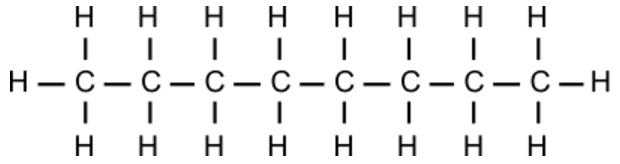
\includegraphics[width=300px]{Figures/Prerequis/developpee.png}
    \caption{\label{dev}Formule développée de la molécule d'octane.}
  \end{center}
\end{figure}

L'ensemble du manuscrit est orienté vers l'étude de molécules issues de constructions biologiques.
Une molécule peut classiquement être représentée en 2D sous la forme d'un dessin d'atomes représentés par des lettres, liées par des traits représentant les liaisons covalentes entre atomes (voir figure \ref{dev}).
Cette représentation est appelée \textit{formule développée} de la molécule.

\begin{figure}[h!]
  \begin{center}
    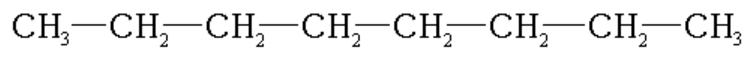
\includegraphics[width=300px]{Figures/Prerequis/semi.png}
    \caption{\label{semi}Formule semi-développée de la molécule d'octane.}
  \end{center}
\end{figure}

Les atomes d'hydrogène étant omniprésents, la représentation de grandes molécules peut aboutir sur une formule développée volumineuse.
Pour simplifier leur représentation a été inventée la forme dite \textit{semi-développée} (voir figure \ref{semi}).
Puisque les atomes d'hydrogène n'effectuent qu'une seule liaison, la représentation de ceux-ci peut être contracté avec l'atome qu'ils accompagnent, sans pour autant laisser un doute sur les liaisons non représentées.


\section{Représentation 1D d'une molécule : les SMILES}

Les librairies de chemoinformatique utilisent réguliérement un format plus compact pour les représentations moléculaires.
Toute la structure est alors compactée en un texte.
Ce format est appelé SMILES (pour \textit{Simplified Molecular Input Line Entry Specification}) et a été publié en 1988~\cite{weininger_smiles_1988}.
L'octane représenté en figures \ref{dev} et \ref{semi} peut par exemple être écrit sous la forme verbeuse du SMILES :

\[\text{[C]([H])([H])([H])[C]([H])([H])[C]([H])([H])[C]([H])([H])[C]([H])([H])[C]([H])([H])}\]
\[\text{[C]([H])([H])[C]([H])([H])[H]}\]

Chaque atome est ici représenté par une lettre entourée de crochets.
% Deux atomes directement à la suite l'un de l'autre sont considérés comme liés.
Toute sous partie de l'expession mise entre parenthèses représente un embranchement à partir de l'atome précédent.
Sur cet exemple, la chaîne principale est donc constituée de [C][C][C][C][C][C][C][C][H].
Chacun des [C] est accompagné de plusieurs branchements ne contenant qu'un seul hydrogène.
Par exemple le début de la chaîne est constituée d'un [C]([H])([H])([H]), ce qui veut dire que que le premier carbone, en plus d'être lié au carbone suivant, possède trois branches constituées d'un unique hydrogène.
Il est à noter qu'il existe de nombreux SMILES pour représenter cette molécule.
J'ai arbitrairement choisi de commencer par le carbone le plus à gauche de la figure \ref{semi}, mais j'aurais aussi bien pu démarrer de n'importe que atome plus au centre.

La notation présentée est lourde mais deux règles supplémentaires viennent réduire la notation.
Premièrement, les atomes d'hydrogène sont facultatifs.
Même si ils ne sont pas présents dans l'écriture, ils seront automatiquement ajoutés jusqu'à saturation de la valence des atomes hôtes.
Deuxièmement, il est autorisé de ne pas mettre les crochets pour les atomes les plus fréquemment utilisés en chimie organisque (par exemple C, N ou O).
Avec ces deux assouplissements, notre molécule d'octane s'écrirait donc de la manière suivante : CCCCCCCC.

Les SMILES doivent inclure plusieurs autres règles pour pouvoir représenter l'intégralité des molécules possibles.
Ainsi, un = ou un \# sont ajoutés entre deux atomes pour représenter des liaisons doubles ou triples.
Par exemple, le SMILES C(=O)OH représente un groupement carboxyle.
Le =O est une branche, contenant un unique atome d'oxygène, reliée au carbone par une double liaison.

\begin{figure}[h!]
  \begin{center}
    
\includegraphics[width=350px]{Figures/Prerequis/glucose.png}
    \caption{\label{glucose}Molécule de glucose et son ordre de parcours dans le SMILES cyclique exemple.}
  \end{center}
\end{figure}

Les molécules peuvent également être cycliques.
Il n'est pas possible de représenter un cycle dans un texte sans ajouter une notation supplémentaire.
Ainsi, on ajoute un nombre à la suite de chacun des deux atomes distants dans la chaîne de caractère, mais reliés dans la molécule.
La molécule de glucose représentée sur la figure \ref{glucose} s'écrira donc OCC1C(O)C(O)C(O)C(O)O1.
La valeur 1 permet de représenter la liaison entre l'atome d'oxygène dans le cycle et le carbone juste à sa gauche.

Je n'ai décrit ici que les règles qui nous seront utiles.
L'intégralité des spécifications est disponible en ligne sur de nombreux sites.



\section{Graphes}
\label{graphes}

\begin{figure}[h!]
  \begin{center}
    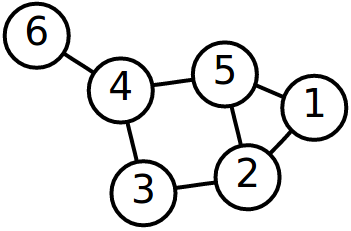
\includegraphics[width=180px]{Figures/Prerequis/graphe.png}
    \caption{\label{graphe_def}Exemple de graphe non orienté contenant 5 noeuds.}
  \end{center}
\end{figure}

Un graphe est un outil permettant de représenter des données sous la forme de n\oe{}uds reliés par des arcs lorsque ceux-ci sont orientés ou par des arêtes pour les non orientés (exemple sur la figure \ref{graphe_def}).
Les n\oe{}uds des graphes peuvent être étiquetés ou non.
Sur l'exemple chaque étiquette de n\oe{}ud est représentée par une couleur.
Le n\oe{}ud 1 est étiqueté par ``bleu'', les n\oe{}uds 2, 3 et 5 par ``vert'' et enfin le n\oe{}ud 4 par ``rouge''.
Dans la suite du manuscrit, nous utiliserons souvent cette représentation colorée des étiquettes pour plus de clarté.

Cette représentation de données est très souvent utilisée en informatique et ce, pour tous type de domaines.
Dans notre cas nous allons l'utiliser à de multiples reprises, et en particulier pour représenter les molécules sous leur forme atomique ainsi que sous leur forme biologique.
Nous verrons dans le second chapitre qu'il est possible de transformer nos molécules en graphes atomiques non orientés dont chacun des noeuds est étiqueté avec des informations sur les atomes.
Cette représentation nous permettra d'appliquer des algorithmes classiques à nos données particulières.





























